\subsection{Results}\label{subsection:results}
After giving a detailed description of the used methodology in the previous subsection this subsection contains the interviews outcome. First the general questions about the interviewees background are evaluated and interpreted. Because this part was included in all three questionnaires, this part also includes data from the other reports for comparing the data, but only the data from the researcher interviews are interpreted. In the next parts, the use case of the library data and publication data are evaluated and their potential benefits, barriers and disadvantages analyzed. In the last part, the ideas and mentions from the open questions are evaluated.

\subsubsection{General statistically evaluation of the interviewees background}\label{stat_general}

\begin{figure}[htbp]
\centering
\label{Fi:lod-exp}
	\begin{tikzpicture}
		\begin{axis}
			[title=Level of ICT-Expertise,
			ybar,% Balken
			% urspr�ngliche y-Werte unterhalb der Balken:
			nodes near coords,nodes near coords align=above,point meta=rawy,
			axis x line=bottom, axis y line=left,% Achsen nur unten und links,
			%xlabel=blub,ylabel=bla, % Beschriftung der Achsen
			ymin=0,% minimaler y-Wert ist 0
			xtick=data,% xticks nur an Stellen mit Daten
			enlargelimits=auto,% Vergr��ern der R�nder des Diagramms
			% Ausgabe der x Werte ohne Tausendermarkierung@
			x tick label style={/pgf/number format/1000 sep=},
			legend pos=north west]
			\addplot table[x=Question, y=Number] {data/data_general_researcher_1.csv};
			\addplot table[x=Question, y=Number] {data/data_general_students_1.csv};
			\addplot table[x=Question, y=Number] {data/data_general_admin_1.csv};
			\legend{Researcher, Students, Administration}
		\end{axis}
	\end{tikzpicture}
	\begin{tikzpicture}
		\begin{axis}		
			[title=Level of LOD-Expertise,
			ybar,% Balken
			% urspr�ngliche y-Werte unterhalb der Balken:
			nodes near coords,nodes near coords align=above,point meta=rawy,
			axis x line=bottom, axis y line=left,% Achsen nur unten und links,
			%xlabel=blub,ylabel=bla, % Beschriftung der Achsen
			ymin=0,% minimaler y-Wert ist 0
			xtick=data,% xticks nur an Stellen mit Daten
			enlargelimits=auto,% Vergr��ern der R�nder des Diagramms
			% Ausgabe der x Werte ohne Tausendermarkierung@
			x tick label style={/pgf/number format/1000 sep=},
			legend pos=north east]
			\addplot table[x=Question, y=Number] {data/data_general_researcher_2.csv};
			\addplot table[x=Question, y=Number] {data/data_general_students_2.csv};
			\addplot table[x=Question, y=Number] {data/data_general_admin_2.csv};
			\legend{Researcher, Students, Administration}
		\end{axis}
	\end{tikzpicture}
	\caption[Level of Experience]{Level of Experience}
\end{figure}

The first part of the interview aimed to categorize the interview partners and to understand their background. They had to estimate their level of expertise in the field of Information \& Communication Technologies and in the field of Linked Open Data in a formal way and then describe their daily work and responsibilities at the university. This part was identical in all three interview series (administration, students and researcher), so the result can be compared. The levels of expertise can be seen in figure~\ref{Fi:lod-exp} and the according rating scales in table~\ref{table:rating-scales}. For a detailed description of the administration and student interviews see the corresponding reports~\citet{article:gamerith_publishing_2016} (administration data) and ~\citet{article:haller_publishing_2016}(data concerning students).

Tough all four research-interviewees had a high expertise in ICTs, their expertise in LOD are mainly unincisive, although everyone already knew the concept of LOD. This can easily explained by their research fields (see table~\ref{table:interviewee-background}): everyone works in a technical context. 

This could be seen as advantage as well as disadvantage. On the one hand the interviewed persons needed lesser effort to understand the benefits of LOD and could easier imagine further use-cases and possible data sets for LOD. But on the other hand, their perspectives were in some way restricted by their profession - a more divergent angle of view may be interesting for further studies to explore more ``non-technical'' use-cases. But for an initial study like this one it may be enough.

	
\begin{figure}[htbp]
  \centering
	\label{table:rating-scales}
	\begin{tabular}{ c | l  | p{10cm} }
		\textbf{Value} & \textbf{ICT} & \textbf{LOD}\\			\hline
		1 & Fundamental & I never heard of Linked Open Data.\\ \hline		
		2 & Novice & I heard of Linked Open Data, but never used it.\\		\hline
		3 & Intermediate & I used Linked Open Data in a not intense way. E.g. as part of a workshop or home project.\\		\hline
		4 & Advanced & I used Linked Open Data in a practical project.\\		\hline
		5 & Expert & I used Linked Open Data in several practical projects and consider myself an expert in Linked Open Data.\\
	\end{tabular}
	\caption[Rating scales]{Rating scales for the level of expertise in the field of ICT and LOD.}
\end{figure}

\begin{figure}[htbp]
  \centering
	\label{table:interviewee-background}
	\begin{tabular}{ c | l | c }
		\textbf{ID} & \textbf{Assignment} & \textbf{Date of interview} \\ \hline
		A & research \& teaching in HCI & 15.12.2015\\
		B & research in information retrieval & 04.12.2015\\
		C & research transfer & 23.11.2015\\
		D & research in audio and video analysis & 24.11.2016\\
	\end{tabular}
	\caption[Interviewees background]{Background information of the interviewees and the corresponding interviews.}
\end{figure}

\subsubsection{General results}\label{subsubsection:general_results}
In this section we describe general results which not applied to one of the described use cases. This mainly involved the common attitudes, thoughts and doubts for LOD of the interviewed persons. 

\subsubsubsection{General benefits}~\label{subsubsubsection:general_benefits}
All interview partners strongly welcomed the idea of LOD and LOD application at the university. Everyone of them could imagine a LOD project despite of possible challenges or problems, they rated clearly the benefits over them. The opportunity to develop new ideas based on an access to open data was very common liked across all questions. One important point was to divide and free the data from their original purpose and application to create context-independent ideas. It was suggested to publish as many data as possible as LOD and then let (master) students in courses and projects make application based on this data without strict restrictions and goals. 

\subsubsubsection{General challenges}
One of the most frequently mentioned challenges was costs in terms of money and work, followed by data quality and administration.

Costs in term of money may be a small challenge if a LOD project stays at a local university context but may raise proportional if the project move to a higher level like Austria- or Europe-wide. In terms of work the challenges are mainly bureaucracy to manage the project and in the maintenance of a living system. This has also a strong connection to the challenge of data quality, a crucial point of real time LOD. If they get outdated, they get useless and therefore a huge investigation of time and work has be done in this area to ensure a high quality of the data. 

Another mentioned challenge was the communication between technically experienced stakeholders and lesser experienced stakeholders which hold the domain knowledge. Therefore a proper ontology must be found to fit both needs and simultaneously describes the data sufficiently. Also this ontology has to be maintained to always fit the needs and data appropriately.

Further some of the interviewees pointed out the way of making the LOD available. To stimulate and motivate other people to work with the data interfaces, they have to know that they exists. Furthermore it won't be successful to just put the data to an endpoint, instead the students, other stakeholder and interested people need to actively be informed about the benefits and availability (e.g. in a way described in the previous section~\ref{subsubsubsection:general_benefits}.

\clearpage 

\subsubsection{Library data}

\paragraph{Use case}
This question aimed for a use case similar to the LD4L project (described in Section ~\ref{ld-libraries}). The proposed scenario was to publish the data or meta-data of the university library (and all of its specialized libraries) as LOD and provide an application to access the data. A further option of this scenario would be an interlinking to other LOD data sets, e.g. from the publisher ``Springer''~\footnote{\url{http://lod.springer.com/data/search}} or to other universities like LD4L do it.

\begin{figure}[htbp]
\centering
\label{Fi:lib-data}
	\begin{tikzpicture}
		\begin{axis}		
			[title=Usefulness of library (meta-)data as LOD,
			ybar,% Balken
			% urspr�ngliche y-Werte unterhalb der Balken:
			nodes near coords,nodes near coords align=above,point meta=rawy,
			axis x line=bottom, axis y line=left,% Achsen nur unten und links,
			%xlabel=blub,ylabel=bla, % Beschriftung der Achsen
			ymin=0,% minimaler y-Wert ist 0
			xtick=data,% xticks nur an Stellen mit Daten
			enlargelimits=auto,% Vergr��ern der R�nder des Diagramms
			% Ausgabe der x Werte ohne Tausendermarkierung@
			x tick label style={/pgf/number format/1000 sep=}]
			\addplot table[x=Question, y=Number] {data/data_ld_library_useful.csv};
		\end{axis}
	\end{tikzpicture}
		\begin{tikzpicture}
		\begin{axis}		
			[title=Imagine at TUVienna? Would use it?,
			ybar,% Balken
			% urspr�ngliche y-Werte unterhalb der Balken:
			nodes near coords,nodes near coords align=above,point meta=rawy,
			axis x line=bottom, axis y line=left,% Achsen nur unten und links,
			%xlabel=blub,ylabel=bla, % Beschriftung der Achsen
			ymin=0,% minimaler y-Wert ist 0
			symbolic x coords = {{No, Yes}},
			xtick=data,% xticks nur an Stellen mit Daten
			enlargelimits=auto,% Vergr��ern der R�nder des Diagramms
			% Ausgabe der x Werte ohne Tausendermarkierung@
			x tick label style={/pgf/number format/1000 sep=},
			legend pos=north west]
			\addplot table[x=Answer, y=Imagine] {data/data_ld_library_use.csv};
			\addplot table[x=Answer, y=Use] {data/data_ld_library_use.csv};
			\legend{Can imagine, Would use}
		\end{axis}
	\end{tikzpicture}
	\caption[Usefulness of library (meta-)data]{Usefulness of library (meta-)data as LOD}
\end{figure}

\paragraph{Statistically evaluation}
It can be seen in Figure~\ref{Fi:lib-data} that the interviewed persons strongly agreed to the scenario (found it ``extremely useful'') and could imagine a similar project at the TU Vienna. Only one interviewee found it difficult to see advantages and therefore argued that he wouldn't use it. He argued that this use case is already covered by Google Scholar~\footnote{\url{https://scholar.google.at/}}. Another one found it indeed useful in a general context but not for his own work.

\paragraph{Needs, potential benefits}
As stated, all of the interviewed persons could imagine a similar project. One of the main reasons of the strong acceptance was the current interface of the library website~\footnote{\url{www.ub.tuwien.ac.at/}}, which only allows a search with only a few, specified parameters (see Figure~\ref{Fi:UB_TU}). Also the physical search in the library itself was claimed due to a lack of orientation and knowledge about the position of e.g. a searched book. Both point of criticism are expected to vanish by an open access to the data and appropriate applications, which provides a detailed and personalizable search interface.

Furthermore an open access to the data was seen as a chance for everyone to interact with it and as opportunity to stimulate creativity of the people.

\paragraph{Notes}
For an implementation of such a LOD system of the library data the Union of Libraries and Service GmbH (OBVSG)~\footnote{\url{www.obvsg.at}} needs to be involved because of the membership of the university library. They manage and maintain the information systems and data stock.

\paragraph{Barriers, potential disadvantages}

The library institution was very conservative perceived with skepticism, refusals and resentment against new ideas, especially in a technical term. It was stated by some interviewees, that this kind of project would only be seen as an extra amount of work in the library and not as an opportunity.

Beside the expected opposition there was also a real amount of work estimated by the interviewees. In particular there would be an effort to invest in digitizing books and keep this data up-to-date. This would be an important part of the project, otherwise the data would lose there value - not digitized data could not be distinguishable from not available data. Therefore it would be essential to have a complete and current database. 

Another concern of the interviewed people were the copyright of the data. However, this problem was seen as handleable, because only meta-data would be open accessible.

At last, one interviewee declined the idea and usefulness of the LD4L and similar projects because of the existing platform Google Scholar~\footnote{\url{https://scholar.google.at/}}. He stated, that it already provides similar data and therefore everything he needs for his work. Further an additional platform would be too intricate to use.

\begin{figure}[htbp]
\centering
\label{Fi:UB_TU}
\subfigure[Homepage and simple search]
{\scalebox{0.3}{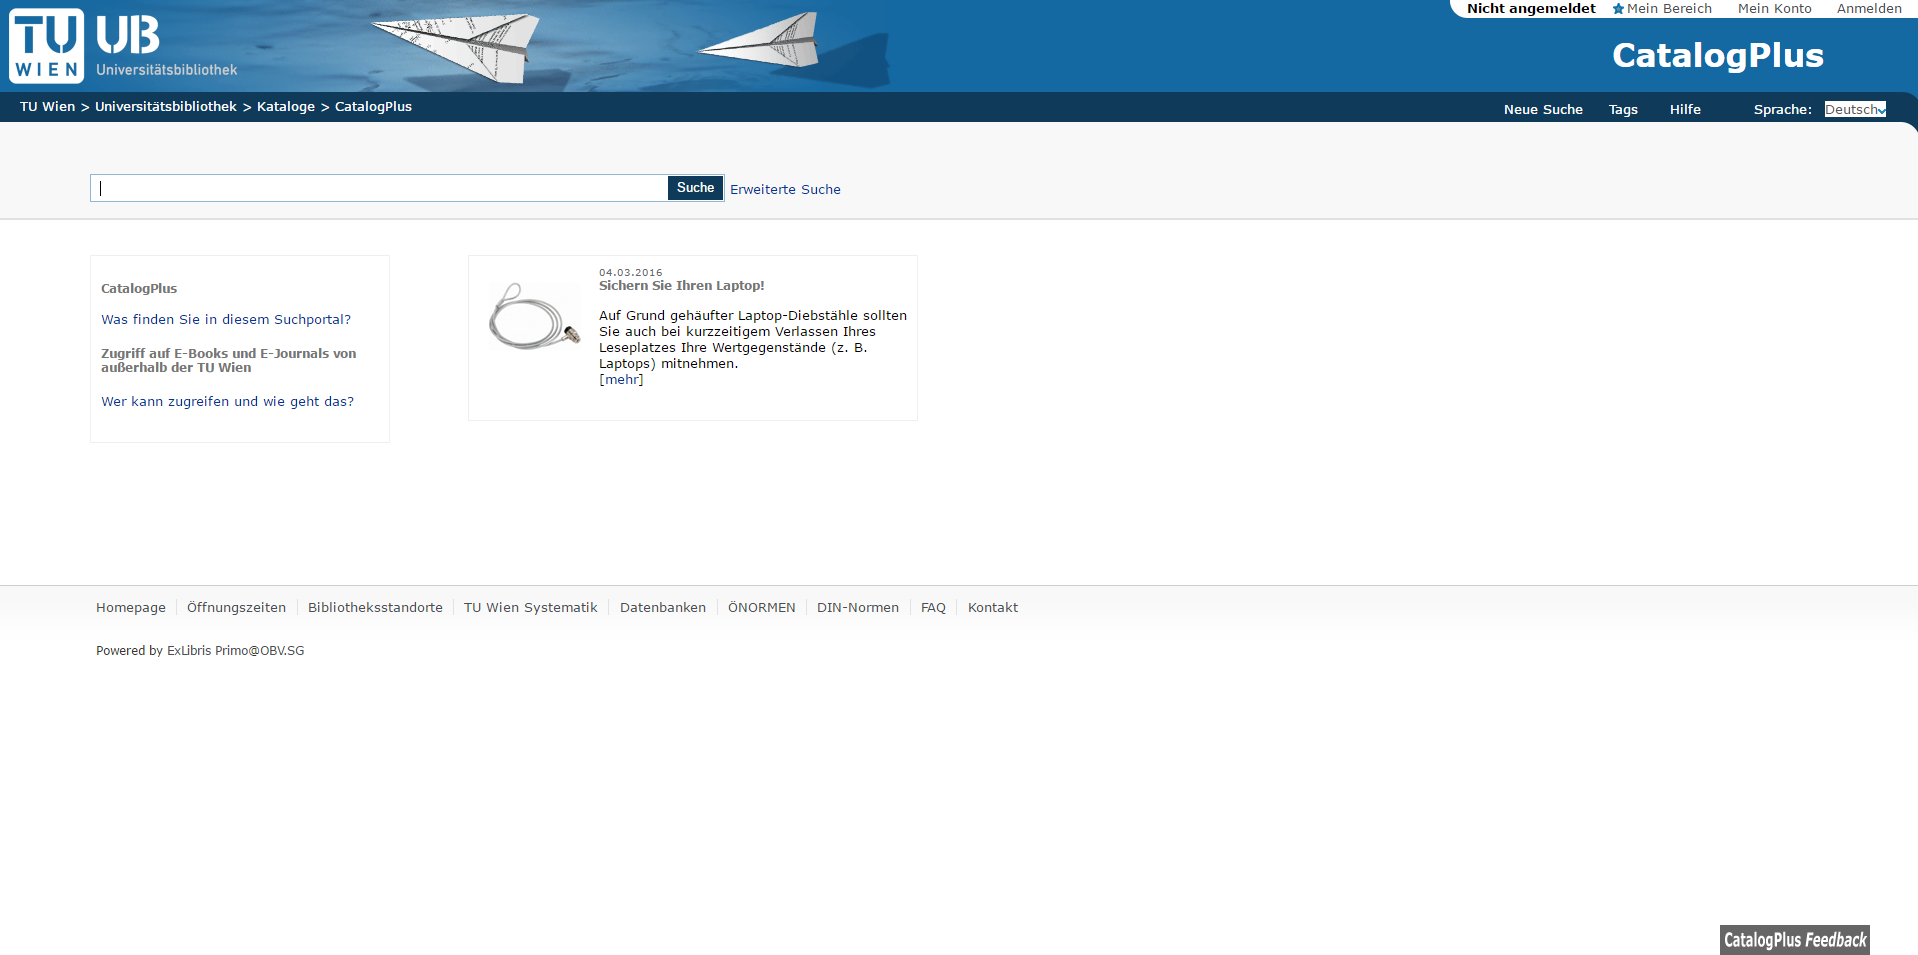
\includegraphics{images/screenshots/screenshot_ub_tu.PNG}}}
\subfigure[Extended search]
{\scalebox{0.3}{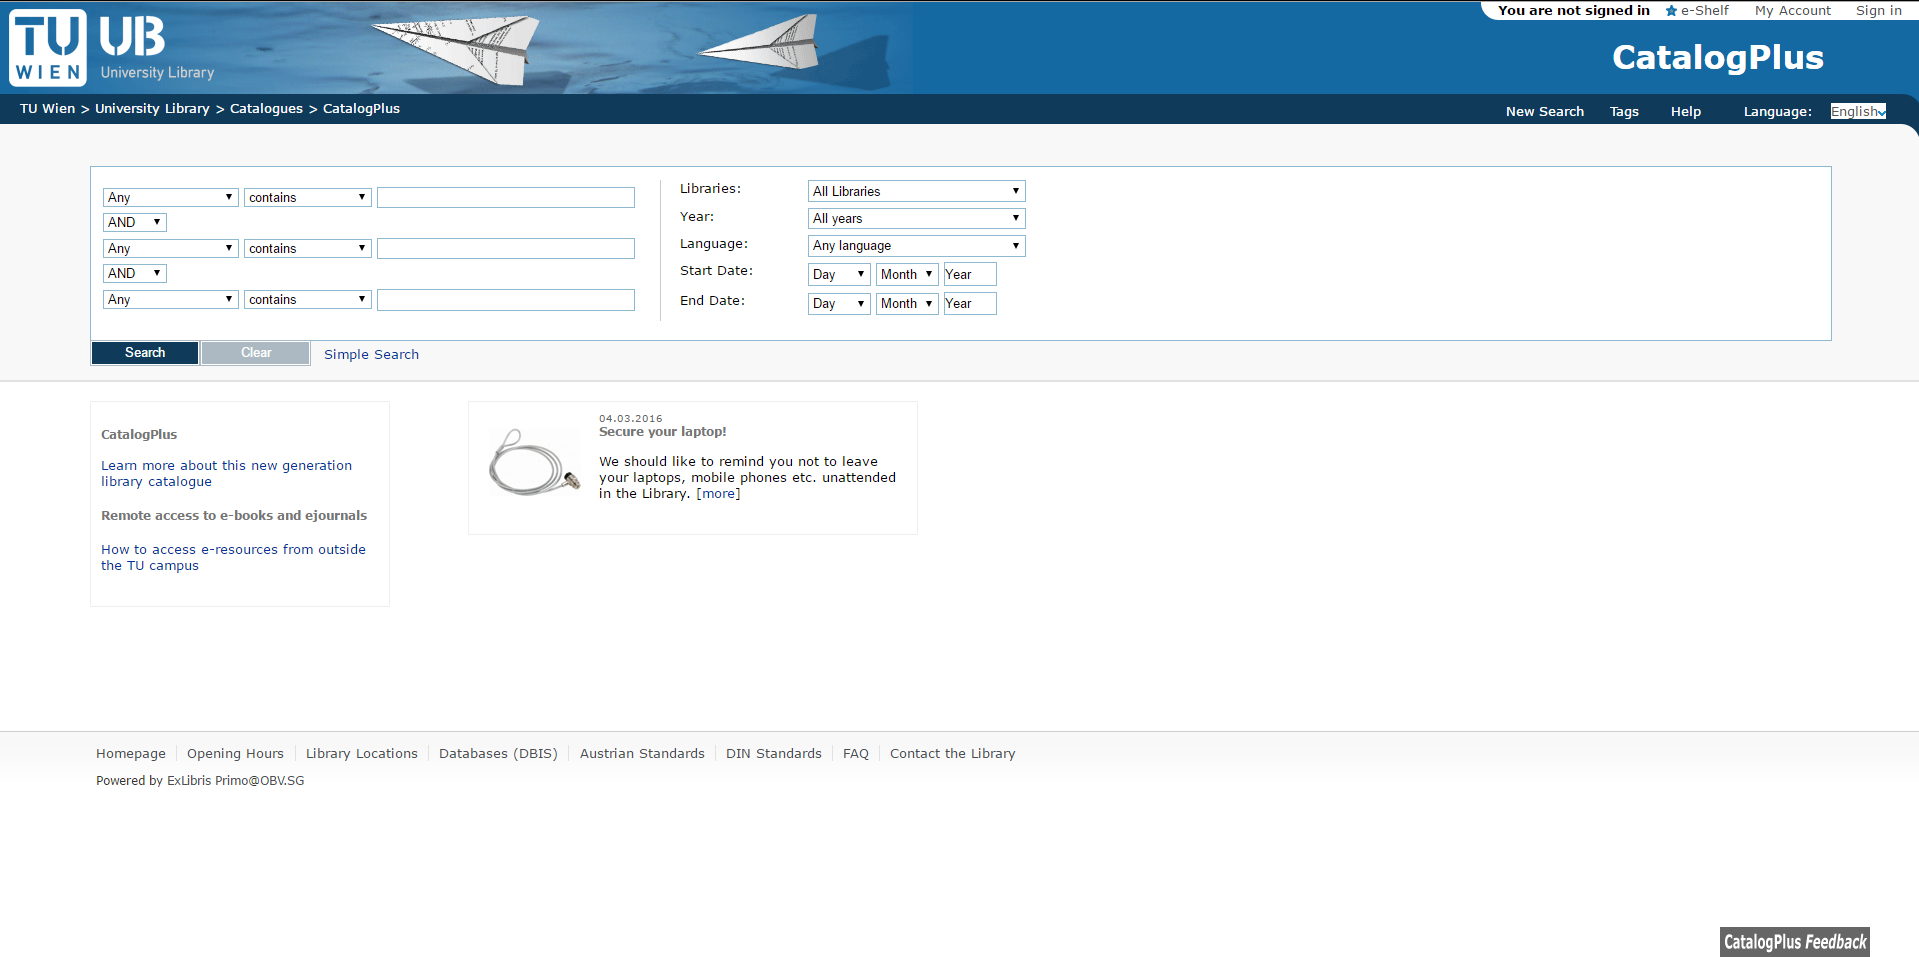
\includegraphics{images/screenshots/screenshot_ub_tu_extended_search.PNG}}}
\caption[Website of the TUVienna library]{Website of the TUVienna library}
\end{figure}

\clearpage 

\subsubsection{Data from the Publication database}

\paragraph{Use case}\label{section:pub_db_usecase}
The proposed use case applied to the already existing publication database of the university. In the current state the database can be accessed via its website~\footnote{\url{www.publik.tuwien.ac.at/pubstart.php}}, where an interface for search exists. For other search parameters a request to the administration has to be made. The introduced LOD approach provides an LOD interface to the existing database, so the data can be accessed over e.g. SPARQL. This use case follows the principle of the existing ``Open Research Online''~\footnote{\url{http://data.open.ac.uk/page/context/oro}} endpoint from the Open University, which expose information about publications originating from OU researchers using the BIBO Ontology (see section~\ref{subsubsec:ontologies} for details).

\begin{figure}[htbp]
\centering
\label{Fi:pub-data}
	\begin{tikzpicture}
		\begin{axis}		
			[title=Usefulness of publication data as LOD,
			ybar,% Balken
			% urspr�ngliche y-Werte unterhalb der Balken:
			nodes near coords,
			nodes near coords align=above,
			point meta=rawy,
			axis x line=bottom, axis y line=left,% Achsen nur unten und links,
			%xlabel=blub,ylabel=bla, % Beschriftung der Achsen
			ymin=0,% minimaler y-Wert ist 0
			xtick=data,% xticks nur an Stellen mit Daten
			enlargelimits=auto,% Vergr��ern der R�nder des Diagramms
			% Ausgabe der x Werte ohne Tausendermarkierung@
			x tick label style={/pgf/number format/1000 sep=}]
			\addplot table[x=Question, y=Number] {data/data_publication_useful.csv};
		\end{axis}
	\end{tikzpicture}
		\begin{tikzpicture}
		\begin{axis}		
			[title=Imagine at TUVienna? Would use it?,,
			ybar,% Balken
			% urspr�ngliche y-Werte unterhalb der Balken:
			nodes near coords,
			nodes near coords align=above,
			point meta=rawy,
			axis x line=bottom, axis y line=left,% Achsen nur unten und links,
			%xlabel=blub,ylabel=bla, % Beschriftung der Achsen
			ymin=0,% minimaler y-Wert ist 0
			symbolic x coords = {No, Yes},
			xtick=data,% xticks nur an Stellen mit Daten
			enlargelimits=auto,% Vergr��ern der R�nder des Diagramms
			% Ausgabe der x Werte ohne Tausendermarkierung@
			x tick label style={/pgf/number format/1000 sep=},
			legend pos=north west]
			\addplot table[x=Answer, y=Imagine] {data/data_publication_use.csv};
			\addplot table[x=Answer, y=Use] {data/data_publication_use.csv};
			\legend{Can imagine, Would use}
		\end{axis}
	\end{tikzpicture}
	\caption[Usefulness of publication data]{Usefulness of publication data as LOD}
\end{figure}

\paragraph{Statistically evaluation}
Similar to the library use case the interviewees liked the idea and found it all ``extremely useful''. Everyone could imagine such a project at TUVienna and would also use it.

\paragraph{Needs, potential benefits}
In contrast to the previous use case, the work amount of work was significant lesser stated, because the data are already there, just as the need of being up-to-date of the database.\newline 
Further some of the interviewed persons (independent to each other) come up with the idea of building an application based on the Linked Open Data interface to provide an overview of a researcher references as a widget or similar for a personal website. The data could be interlinked e.g. with the LOD interface of the Springer publisher~\footnote{\url{www.lod.springer.com/}} and complemented by including the Journal Impact Factor (JIF).

\paragraph{Barriers, potential disadvantages}
The interviewees identified uniformly a problem with the data ownership. Although there is an administration of the database, the \textit{ownership} of the data itself is very unclear and therefore a contact and responsible person would be hard to find for such a project - there needs to be more investigation.\newline
Another point, some of the interviewed persons were concerned of, was quality assurance - to use the data, they need to be synchronized with the original database. To taking care of this point, the implementation of a similar project has to ensure this.

\begin{figure}[htbp]
\centering
\label{Fi:pub_db}
{\scalebox{0.3}{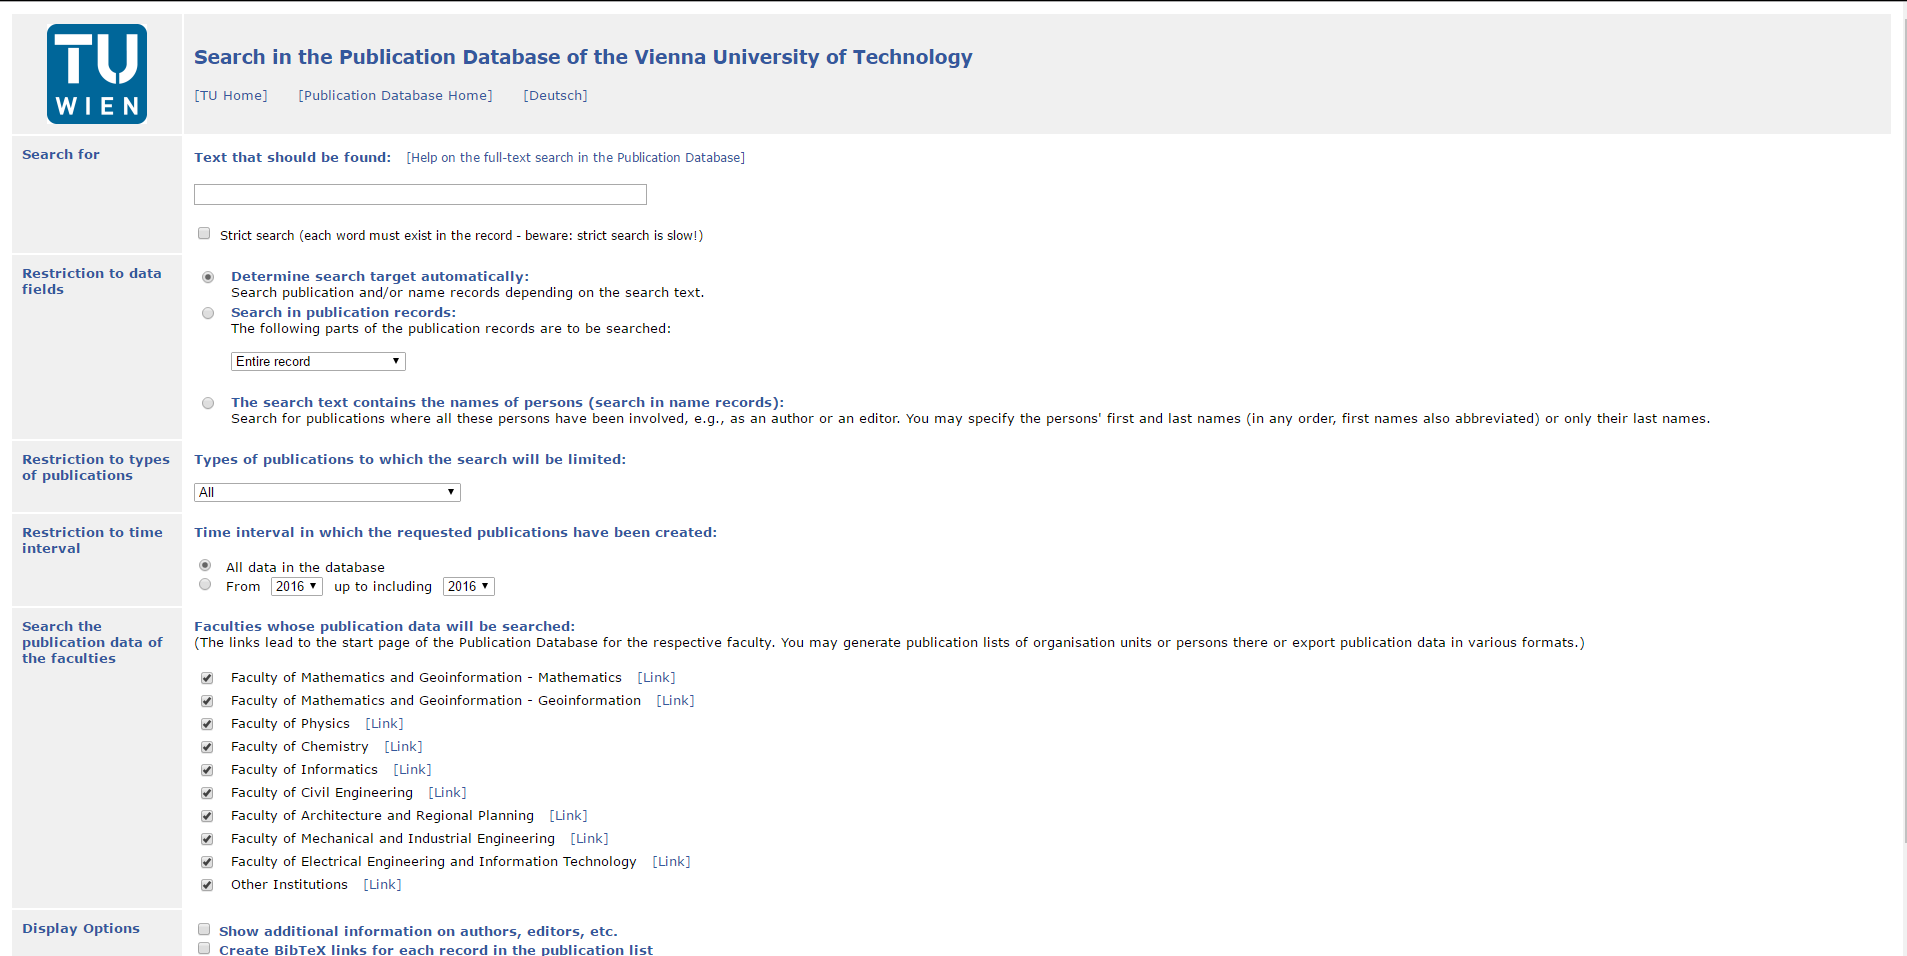
\includegraphics{images/screenshots/screenshot_pub_database.PNG}}}
\caption[Publication database]{Publication database}
\end{figure}

\clearpage 

\subsubsection{Further use cases}~\label{subsubsec:further_use_cases}
In this subsection we describe some other use cases mentioned by the interviewees. Beside the two main use cases described above, some of the interviewees came up with their own ideas. This use cases are results of the flow of conversation, so they may not be fully reasoned, so consider this subsection as some kind of wish list or a collection of what \textit{might} be possible.

\subsubsubsection{``Sideproducts'' of research}
During the most research work a lot of ``sideproducts'' are produced. This can be all kind of statistics, survey data, project descriptions, work documents or sample data. The majority of this data get lost or somewhere stored after the project is done. Though they are evaluated and analyzed during the project, the data may be interesting from other, not intended perspectives - but they are not or only restricted-by-knowledge~\footnote{only available if the existence are known} available. If the data sets would be accessible through a LOD interface, a cross-disciplinary use are imaginable, e.g. a Visual Computing research project could use model data from a architecture research project without detailed knowledge of the original source (which could be gained through links in the LODs). To offer a sufficient data base, this kind of project may be more meaningful in an European context.

Besides the obvious benefits of this use case, there are many challenges and problems. First there has to be implemented a highly flexible LOD-system, which can simultaneously handle a high range of formats (e.g. documents, tables, raw data) and interlink them probably. Further, to make them interlinkable and searchable, there has to be invested a big amount of \textit{manual} work to label the data. The result will be a huge list of keywords, which, again, has to be searchable. Another crucial point are the quality of the labeling: they had to be specific as possible to specify them accordingly as well as general as possible to  free them from the original context and make them interdisciplinary understandable. And, at last, such a system must be as little as possible work to input the data from the project and anonymize them to avoid unnecessary frustration (which could easily overrule the benefits).

\subsubsubsection{Statistics from TISS}
The university management system TISS already provides a lot of statistically data, e.g. 	inscription data or general data about the students, so this data are optimal for a LOD use. The co-work of~\citet{article:haller_publishing_2016} and~\citet{article:gamerith_publishing_2016} explore and evaluate this use case.

\subsubsubsection{Make Curricula comparable}
One big problem of the communication between universities are the missing comparability of their curricula. To determine which university offers which course they have to manually be searched, listed and additionally matched with the corresponding, similar, regarding to the content, but different named courses at other universities. In particular this process is important for reworking the content of study programs to raise the coverage of the research field. Publishing the curricula of the universities as LOD would strongly improve this process and make them comparable. 

Again, this use case makes only sense in an European context, e.g. in corporation with the Erasmus program to simplify the process of course crediting. Though it may be easy to publish single curricula of an university, it adds more profitableness to implement an Europe-wide system.

\subsubsubsection{Overview of university projects and research focuses}
Similar to the use case about the curricula described above, an Europe-wide publishing of university research projects (if they are not under restriction) and research focuses as LOD would be very useful to link researcher with other teams working on similar areas. Such a system could provide a research field based search and allow queries like ``Who is currently working on non-classical logics in Europe?'' or ``Which university has a research focus on artificial social intelligence?''.

This information may not only be interesting for researcher but also for companies, which looking for corporations, or scientific funding.